% =====================================================================
%  Lab 1 -- Market Study
%  ZoneSense: Smart Zone Environmental Monitoring and HVAC Control System
% =====================================================================
\documentclass[11pt,a4paper]{article}
% =====================================================================
%  ZoneSense lab reports -- shared preamble
%  CS3151 Software Engineering, Effat University, Fall 2026
%  Compiler: pdfLaTeX (Overleaf default)
% =====================================================================

% ---------- Fonts and encoding ----------
\usepackage[T1]{fontenc}
\usepackage[utf8]{inputenc}
\usepackage{lmodern}               % Latin Modern for typewriter text
\usepackage{mathptmx}              % Times for body text
\usepackage[scaled=0.90]{helvet}   % Helvetica for table headers and captions
\usepackage{textcomp}
\usepackage{amssymb}
\usepackage{microtype}

% ---------- Page layout ----------
\usepackage[a4paper,top=2.2cm,bottom=2.2cm,left=2.2cm,right=2.2cm,headheight=16pt]{geometry}
\setlength{\parindent}{0pt}
\setlength{\parskip}{6pt plus 1pt}
\linespread{1.08}
\setlength{\emergencystretch}{2em}

% ---------- Colours (taken from the SRS) ----------
\usepackage[table]{xcolor}
\definecolor{znavy}{HTML}{173A5E}   % headings, table headers
\definecolor{zteal}{HTML}{1A9EAD}   % sub-headings
\definecolor{zrow}{HTML}{F0F5FA}    % alternating table rows
\definecolor{zline}{HTML}{B7C6D5}   % table rules
\definecolor{znote}{HTML}{FFF6DB}   % call-out background
\definecolor{znotebar}{HTML}{D9A21B}% call-out bar
\definecolor{zpink}{HTML}{FBEDED}
\definecolor{zmint}{HTML}{E3F4F1}
\definecolor{zgreen}{HTML}{1E7B3A}
\definecolor{zcode}{HTML}{F5F7F9}

% ---------- Packages ----------
\usepackage{graphicx}
\usepackage{array}
\usepackage{tabularx}
\usepackage{xltabular}
\usepackage{makecell}
\usepackage{enumitem}
\usepackage{titlesec}
\usepackage{fancyhdr}
\usepackage{float}
\usepackage{caption}
\usepackage{needspace}
\usepackage[most]{tcolorbox}
\usepackage{listings}
\usepackage{xurl}
\usepackage[hidelinks]{hyperref}
\urlstyle{same}

\graphicspath{{figures/}}

% ---------- Headings ----------
\setcounter{secnumdepth}{3}
\titleformat{\section}{\LARGE\bfseries\color{znavy}}{\thesection.}{0.5em}{}
\titleformat{\subsection}{\Large\bfseries\color{zteal}}{\thesubsection}{0.6em}{}
\titleformat{\subsubsection}{\large\bfseries\color{znavy}}{\thesubsubsection}{0.6em}{}
\titleformat{\paragraph}[runin]{\normalsize\bfseries\color{znavy}}{}{0pt}{}
\titlespacing*{\section}{0pt}{6pt}{12pt}
\titlespacing*{\subsection}{0pt}{14pt}{6pt}
\titlespacing*{\subsubsection}{0pt}{12pt}{4pt}
\titlespacing*{\paragraph}{0pt}{8pt}{0.6em}

% ---------- Lists ----------
\setlist{itemsep=2pt,topsep=3pt,parsep=0pt}

% ---------- Tables ----------
\newcolumntype{L}[1]{>{\raggedright\arraybackslash}p{#1}}
\newcolumntype{C}[1]{>{\centering\arraybackslash}p{#1}}
\newcolumntype{Y}{>{\raggedright\arraybackslash}X}
\newcolumntype{B}[1]{>{\raggedright\arraybackslash\leavevmode\bfseries\color{znavy}}p{#1}} % bold navy first column
\newcolumntype{Z}{>{\centering\arraybackslash}X}
\renewcommand{\arraystretch}{1.25}
\setlength{\tabcolsep}{5pt}
\arrayrulecolor{zline}
\newcommand{\hd}[1]{\leavevmode\textcolor{white}{\sffamily\bfseries #1}}   % header cell
\newcommand{\headrow}{\rowcolor{znavy}}                            % header row
\newcommand{\stripe}{\rowcolors{2}{white}{zrow}}                    % zebra rows

% ---------- Captions ----------
\captionsetup{font={small,sf},labelfont={bf,color=znavy},textfont={bf,color=znavy},
  labelsep=endash,justification=raggedright,singlelinecheck=false,skip=4pt}
\captionsetup[figure]{font={small,sf},labelfont={color=gray},textfont={color=gray},
  justification=centering,singlelinecheck=true,skip=6pt}

% ---------- Handy macros ----------
\newcommand{\COtwo}{CO\textsubscript{2}}
\newcommand{\tick}{\ensuremath{\checkmark}}
\newcommand{\gtick}{\textcolor{zgreen}{\ensuremath{\checkmark}}}
\newcommand{\cbox}{\ensuremath{\square}}

% Call-out box (yellow, left bar) -- used for notes in the SRS
\newtcolorbox{zcallout}{enhanced,breakable,colback=znote,colframe=znote,
  borderline west={3pt}{0pt}{znotebar},arc=0pt,outer arc=0pt,
  left=8pt,right=8pt,top=5pt,bottom=5pt,fontupper=\small,before skip=8pt,after skip=8pt}

% Light-blue information box
\newtcolorbox{zinfo}{enhanced,colback=zrow,colframe=zrow,arc=0pt,outer arc=0pt,
  left=8pt,right=8pt,top=6pt,bottom=6pt,fontupper=\small,before skip=8pt,after skip=8pt}

% Code listings
\lstset{basicstyle=\ttfamily\scriptsize,columns=fullflexible,keepspaces=true,
  breaklines=true,breakatwhitespace=false,showstringspaces=false,upquote=true,
  frame=single,rulecolor=\color{zline},backgroundcolor=\color{zcode},
  xleftmargin=4pt,xrightmargin=4pt,framexleftmargin=4pt,framexrightmargin=4pt,
  aboveskip=8pt,belowskip=8pt,tabsize=4,
  literate={≤}{{$\le$}}1 {≥}{{$\ge$}}1 {→}{{$\rightarrow$}}1 {–}{{--}}1}

% ---------- Header and footer ----------
\pagestyle{fancy}
\fancyhf{}
\fancyhead[L]{\small\sffamily\textcolor{znavy}{\ShortTitle}}
\fancyhead[R]{\small\sffamily\textcolor{gray}{CS3151 -- Software Engineering}}
\fancyfoot[L]{\footnotesize\sffamily\textcolor{gray}{CS3151/2026 \quad Dr.\ Passent Elkafrawy}}
\fancyfoot[R]{\footnotesize\sffamily\textcolor{gray}{\thepage}}
\renewcommand{\headrulewidth}{0.4pt}
\renewcommand{\headrule}{\hbox to\headwidth{\color{zline}\leaders\hrule height \headrulewidth\hfill}}

% ---------- Cover page ----------
% Set \LabTitle, \ProjectTitle and \TeamMembers in main.tex before \begin{document}.
\newcommand{\makecover}{%
  \begin{titlepage}
    \centering
    \vspace*{1.2cm}
    
\includegraphics[width=3.6cm]{effat_logo.png}\par
    \vspace{1.6cm}
    {\Large\bfseries Course: CS3151 -- Software Engineering\par}
    \vspace{0.35cm}
    {\large\bfseries Project -- Fall 2026\par}
    \vspace{0.15cm}
    {\large\bfseries Instructor: Dr.\ Passent Elkafrawy\par}
    \vspace{1.6cm}
    {\large\bfseries \ProjectTitle\par}
    \vspace{0.9cm}
    {\color{znavy}\rule{0.55\linewidth}{0.6pt}\par}
    \vspace{0.45cm}
    {\LARGE\bfseries\color{znavy} \LabTitle\par}
    \vspace{0.35cm}
    {\color{znavy}\rule{0.55\linewidth}{0.6pt}\par}
    \vfill
    {\large\bfseries Done By:\par}
    \vspace{0.4cm}
    {\large \TeamMembers\par}
    \vspace{2.2cm}
  \end{titlepage}%
}

% Keep a run-in heading together with the text that follows it
\newcommand{\keephead}[1]{\needspace{6\baselineskip}\paragraph{#1}\leavevmode\par\vspace{-\parskip}}

% Never leave a heading stranded at the bottom of a page
\usepackage{etoolbox}
\pretocmd{\section}{\needspace{8\baselineskip}}{}{}
\pretocmd{\subsection}{\needspace{6\baselineskip}}{}{}
\pretocmd{\subsubsection}{\needspace{5\baselineskip}}{}{}


\newcommand{\ShortTitle}{ZoneSense -- Lab 1: Market Study}
\newcommand{\LabTitle}{Lab 1: Market Study}
\newcommand{\ProjectTitle}{ZoneSense: Smart Zone Environmental Monitoring and HVAC Control System}
\newcommand{\TeamMembers}{%
  Remas Rawas --- ID: S24109161\\[6pt]
  Bayan Abduldaym --- ID: S24109196\\[6pt]
  Ghala Bin Salim --- ID: S24109159}

\counterwithin{table}{section}
\counterwithin{figure}{section}

% Company box used in Section 2.2.1
\newtcolorbox{company}[2]{enhanced,colback=white,colframe=zline,boxrule=0.4pt,arc=0pt,outer arc=0pt,
  colbacktitle=#1,coltitle=zteal,fonttitle=\bfseries\large,title={#2},
  left=6pt,right=6pt,top=4pt,bottom=4pt,before skip=6pt,after skip=8pt}

\begin{document}
\makecover

% ---------------------------------------------------------------------
\section{Introduction, Problem Statement \& Project Scope}

\subsection{Introduction}
ZoneSense is a proposed Smart Zone Environmental Monitoring and Heating, Ventilation, and Air Conditioning (HVAC) Control System designed to support environmental monitoring and facility management within a single building.

The proposed system will monitor temperature, carbon dioxide (\COtwo), humidity, and sound levels across up to 20 monitoring zones. The limit of 20 monitoring zones is defined as a project-scope boundary to keep the academic prototype manageable while still representing a multi-zone building environment; it is not intended to represent the technical maximum capacity of the system. It will provide Building Residents and HVAC Maintenance Technicians with information to identify abnormal environmental conditions and support appropriate responses.

\subsection{Problem Statement}
Facility management teams may face challenges when monitoring environmental conditions across multiple building zones. Environmental readings may be difficult to interpret collectively, making it harder to identify which zones require immediate attention.

Abnormal temperature, \COtwo, humidity, or sound levels may not be recognized promptly. Additionally, HVAC Maintenance Technicians may lack sufficient zone-specific information before investigating environmental or equipment-related incidents.

The proposed ZoneSense system aims to address these challenges through centralized environmental monitoring, clear zone-status indicators, abnormal-condition alerts, and a human-supervised response workflow.

\subsection{Project Scope}
ZoneSense will collect and store environmental sensor readings and evaluate them against configured thresholds. Each monitoring zone will be assigned one of four statuses: normal, warning, critical, or unavailable.

When an environmental reading violates a configured threshold, the system will generate an alert identifying the affected zone, abnormal measurement, current reading, and severity.

For controllable abnormal temperature, \COtwo, or humidity conditions, ZoneSense will propose a supported HVAC control action. Every proposed control action will require explicit approval from an authorized Building Resident before execution. Rejected actions will not be executed.

Abnormal sound levels will trigger alerts for investigation rather than HVAC control actions. The system will also support maintenance activity recording, historical records, user authentication, and role-based access control.

The initial project scope will be limited to one building with up to 20 monitoring zones, consistent with the defined academic prototype boundary. The academic prototype may use simulated sensor readings and HVAC control actions, while integration with physical building equipment will depend on supported interfaces and site-specific compatibility.

% ---------------------------------------------------------------------
\clearpage
\section*{SDGs and Strategy 2030}
\addcontentsline{toc}{section}{SDGs and Strategy 2030}
{\large\color{znavy} Healthier buildings, smarter cities\par}
\vspace{14pt}

\vspace{6pt}
\begingroup\leftskip=1.2cm
{\Large\bfseries\color{zteal} UN Sustainable Development Goals\par}
\vspace{12pt}
\newcommand{\sdg}[3]{{\color{znavy}\makebox[1.1cm][r]{\Large\bfseries #1}\hspace{8pt}{\large\bfseries #2}\par\vspace{3pt}\hspace*{1.4cm}#3\par\vspace{14pt}}}
\sdg{3}{Good Health and Well-being}{Healthier indoor air through \COtwo{} monitoring and ventilation response}
\sdg{9}{Industry, Innovation and Infrastructure}{Software innovation for smarter building infrastructure}
\sdg{11}{Sustainable Cities and Communities}{Safer, more comfortable and better-managed buildings}
\vspace{16pt}
{\Large\bfseries\color{zteal} Strategy 2030 \textperiodcentered{} Saudi Vision 2030\par}
\vspace{12pt}
\newcommand{\vision}[2]{{\color{znavy}\hspace*{1.4cm}{\large\bfseries #1}\par\vspace{3pt}\hspace*{1.4cm}#2\par\vspace{14pt}}}
\vision{A Vibrant Society}{Healthy, comfortable indoor spaces for people who study and work}
\vision{A Thriving Economy}{Building technology and local software skills}
\vision{An Ambitious Nation}{Accountable operations through roles, approvals and audit records}
\endgroup

% ---------------------------------------------------------------------
\clearpage
\section{Market Study}

\subsection*{Project Description}
The proposed project will be a zone-based environmental monitoring and control system for a single building. The building will be divided into identifiable monitoring zones. Each monitored zone will provide temperature, \COtwo, humidity, and sound-level measurements. The system will present these measurements through a visual interface. It will use clear visual indicators to help users distinguish normal, warning, critical, and unavailable conditions. The system will compare environmental measurements with configured acceptable ranges. If a measurement falls outside its acceptable range, the system will generate an alert. The alert will identify the affected zone and the abnormal environmental condition. For abnormal temperature, \COtwo, or humidity conditions, the system may propose an HVAC-related response when the connected HVAC equipment can affect the detected condition. For example, a proposed response may involve changing temperature control or ventilation. The system will present the proposed action to the Building Resident. The proposed control action will not be executed unless the Building Resident approves it. If the Building Resident rejects the action, the system will not execute it. An abnormal sound level will generate an alert for investigation rather than an HVAC response because the sound-monitoring component measures environmental noise and does not control its source. After an approved action or maintenance activity, the system will continue monitoring the affected zone. New sensor readings will be used to determine whether the environmental condition has changed and to update the zone status.

\subsection{Introduction}
Building management systems are used to monitor indoor environmental conditions and control building equipment such as heating, ventilation, and air conditioning (HVAC). Existing commercial systems provide environmental monitoring, alerts, visualization, and building-control functions. Some systems also provide broader capabilities such as energy management, analytics, integration with other building systems, and multi-building management. These existing solutions demonstrate that environmental monitoring and HVAC control are established technologies. Therefore, the problem addressed by this project is not the absence of building-management technology. The project focuses on the need for a clear and focused workflow for monitoring environmental conditions at the zone level and responding to abnormal conditions under human supervision. The proposed system will focus on a single monitored building divided into environmental zones. It will monitor temperature, carbon dioxide (\COtwo), humidity, and sound level in each zone. It will organize these measurements by zone so that facility staff can understand the current environmental condition of different areas of the building. When an abnormal condition is detected, the system will alert the appropriate user and propose a response. Any proposed control action will require approval from an authorized Building Resident before execution.

\subsection{Competitor Analysis}
The building automation market includes several established systems that provide capabilities related to the proposed project. These capabilities include environmental monitoring, building visualization, HVAC control, and alarm management. Four commercial systems were selected for comparison: Siemens Desigo/Building X, Johnson Controls Metasys, Schneider Electric EcoStruxure Building Operation, and Honeywell Building Management. The comparison examines the capabilities already provided by these systems and identifies how the scope of the proposed system differs from existing solutions.

\subsubsection{Existing Solutions}
\begin{company}{zpink}{Siemens Desigo / Building X}
Siemens Desigo and Building X provide building automation and management capabilities for monitoring and controlling building environments. Desigo supports environmental measurements such as temperature, humidity, and \COtwo{} and integrates these measurements with HVAC control. Siemens also provides centralized visualization and alarm management. Its broader building-management solutions support capabilities beyond the scope of the proposed system, including energy management, analytics, and management across larger building portfolios.
\end{company}

\begin{company}{zmint}{Johnson Controls Metasys}
Johnson Controls Metasys is a building automation system that integrates the monitoring and control of HVAC and other building systems. It monitors environmental conditions such as zone temperature, humidity, and \COtwo. Metasys also provides visualization and alarm-management functions for identifying and managing abnormal conditions. In addition to monitoring, the system can control connected building equipment. It also supports large-scale deployments and integration with building systems beyond the scope of the proposed project.
\end{company}

\begin{company}{zpink}{Schneider Electric EcoStruxure Building Operation}
EcoStruxure Building Operation is a building-management platform for monitoring and controlling connected building systems. It integrates HVAC with other building systems and provides graphical interfaces, dashboards, alarms, and environmental monitoring. Schneider Electric solutions can monitor environmental factors such as temperature, air quality, light, and sound. The platform also provides broader capabilities such as energy management and integration with multiple building systems.
\end{company}

\begin{company}{zmint}{Honeywell Building Management}
Honeywell provides building-management solutions for monitoring and controlling building operations. Its systems support environmental monitoring, HVAC control, dashboards, alerts, and remote building management. Honeywell also provides solutions for managing energy use and multiple connected building systems. These capabilities extend beyond the focused environmental-monitoring scope of the proposed project.
\end{company}

\subsection{Feature Comparison}
The comparison is based on capabilities identified in publicly available product information and documentation. \tick{} indicates that the capability was identified in the reviewed sources. \textit{Partial} indicates that related functionality was identified, but the full capability could not be confirmed. \textit{Not identified} indicates that the capability was not found in the reviewed sources; it does not indicate that the product cannot support it. \textit{Outside project scope} indicates that the capability is provided by existing commercial systems but is not planned for the proposed system.

{\small\stripe
\begin{xltabular}{\linewidth}{|L{3.3cm}|Z|Z|Z|Z|Z|}
\caption{Feature comparison of existing solutions and the proposed system}\label{tab:features}\\
\hline\headrow
\hd{Feature} & \hd{Siemens Desigo / Building X} & \hd{Johnson Controls Metasys} & \hd{Schneider EcoStruxure} & \hd{Honeywell Building Management} & \hd{Proposed System}\\\hline
\endfirsthead
\hline\headrow
\hd{Feature} & \hd{Siemens Desigo / Building X} & \hd{Johnson Controls Metasys} & \hd{Schneider EcoStruxure} & \hd{Honeywell Building Management} & \hd{Proposed System}\\\hline
\endhead
Environmental condition monitoring & \tick & \tick & \tick & \tick & \tick\\\hline
Visual dashboards / building & \tick & \tick & \tick & \tick & \tick\\\hline
Abnormal-condition alerts & \tick & \tick & \tick & \tick & \tick\\\hline
HVAC / building control & \tick & \tick & \tick & \tick & \tick\\\hline
Energy management and optimization & \tick & \tick & \tick & \tick & Outside project scope\\\hline
Multi-building / portfolio management & \tick & \tick & \tick & \tick & Outside project scope\\\hline
Integration with multiple building systems & \tick & \tick & \tick & \tick & Outside project scope\\\hline
Advanced analytics / optimization & \tick & \tick & \tick & \tick & Outside project scope\\\hline
Large-scale deployment & \tick & \tick & \tick & \tick & Outside project scope\\\hline
Focused temperature, \COtwo, humidity, and sound-level workflow & Not identified & Not identified & \tick & Not identified & \tick\\\hline
Mandatory human approval before proposed control actions & Not identified & Not identified & Not identified & Not identified & \tick\\\hline
\end{xltabular}}

The comparison demonstrates that the main technical capabilities of the proposed system, including environmental monitoring, visualization, alerts, and HVAC control, are already available in commercial building-management platforms. These platforms also provide broader capabilities, such as energy management, advanced analytics, multi-building management, and integration with multiple building systems, which are outside the scope of the proposed project. The proposed system will instead focus on a narrower zone-based environmental workflow. It will monitor temperature, \COtwo, humidity, and sound level within individual zones and identify abnormal environmental conditions. When a controllable abnormal condition is detected, the system will propose an appropriate control action. The authorized Building Resident must approve the proposed action before the system executes it.

\subsection{Customer Feedback Analysis}
Public customer reviews of existing building-management products were examined to identify reported strengths and limitations. Because publicly available reviews of specialized building-management software are limited, the findings are used as supporting evidence and do not represent the experiences of all customers.

\subsubsection{Positive Feedback}
Customer reviews of Johnson Controls Metasys highlight centralized monitoring and the ability to integrate and control different building systems. Reviewers identify HVAC control, alarms, remote access, analytics, and system integration as useful capabilities. Reviews of Honeywell building-management solutions also identify centralized building management as a useful capability. Reported benefits include centralized building controls, temperature monitoring, and alerts. Overall, the reviewed customer feedback supports the value of centralized monitoring, building-system control, and timely alerts.

\subsubsection{Negative Feedback and Market Opportunity}
Some Metasys reviewers report limitations related to graphics, user-interface usability, response time, and the initial learning process. A verified EcoStruxure reviewer reported that training was required before becoming comfortable with the system. Some Honeywell customer feedback also identifies cost as a concern. These limitations suggest an opportunity for a more focused system, but they do not indicate that existing commercial platforms lack environmental monitoring or building-control capabilities. Existing platforms provide extensive functionality and support many building-management tasks beyond the scope of the proposed project. The proposed system will therefore focus on a narrower zone-based environmental workflow rather than attempt to reproduce the functionality of a complete commercial building-management platform. It will present temperature, \COtwo, humidity, and sound-level measurements by zone and provide a clear visual indication of each zone's environmental condition. When an abnormal condition is detected, the system will generate an alert. If the condition can be addressed through a supported control action, the system will propose the action to the Building Resident. The action will only be executed after the authorized Building Resident approves it.

This focused scope distinguishes the proposed project from broader commercial platforms without claiming that its individual monitoring, visualization, alert, or control technologies are unique.

\subsection{Market Opportunity \& Differentiation}
The competitor analysis demonstrates an established market for environmental monitoring and building automation. It also shows that the main technologies used by the proposed system are already available in commercial products. These include environmental monitoring, visualization, alarms, HVAC control, and user-authorized building control. Existing commercial platforms also provide broader capabilities, such as energy management, advanced analytics, multi-building management, and integration with multiple building systems.

The proposed system will therefore differentiate itself through its focused scope and response workflow, rather than through individual technologies. It will focus on environmental conditions within zones of a single building. Temperature, \COtwo, humidity, and sound-level measurements will be presented together to provide a clear view of each zone's environmental condition.

When an abnormal condition is detected, the system will generate an alert. If the abnormal condition can be addressed through a supported control action, the system will propose an action to the Building Resident. The system will execute the proposed action only after the authorized Building Resident approves it. Conditions that cannot be addressed through the supported control functions, such as abnormal sound levels, will be reported for investigation rather than automatically associated with an HVAC action.

\begin{zinfo}
{\bfseries\color{zteal} The core workflow is:}\par\smallskip
{\bfseries\color{znavy} Environmental Sensors $\rightarrow$ Zone Monitoring $\rightarrow$ Abnormal-Condition Detection $\rightarrow$ Alert $\rightarrow$ Proposed Control Action (when applicable) $\rightarrow$ Building Resident Approval/Rejection $\rightarrow$ Approved Action Execution $\rightarrow$ Continued Monitoring}
\end{zinfo}

This workflow maintains human authorization over all proposed control actions. The project is intentionally narrower than a full commercial building-management platform and does not attempt to reproduce its broader energy-management, analytics, integration, or multi-building capabilities.

\subsection{Conclusion}
The market study confirms that environmental monitoring and building automation are established areas supported by leading commercial platforms. Siemens, Johnson Controls, Schneider Electric, and Honeywell already provide environmental monitoring, visualization, alarms, HVAC control, and broader building-management capabilities.

The proposed project will not attempt to replace these commercial platforms or claim that its individual technologies are unique. Instead, it will implement a focused, zone-based environmental monitoring and control workflow for a single building. The system will monitor temperature, \COtwo, humidity, and sound level, identify abnormal conditions, generate alerts, and propose supported control actions when applicable. All proposed control actions will require approval from an authorized Building Resident before execution.

The market research therefore supports the relevance of the project while defining its scope as a focused software-engineering solution rather than a comprehensive commercial building-management platform.

% ---------------------------------------------------------------------
\clearpage
\section{Feasibility Analysis}

\subsection{Overview}
The feasibility study evaluates whether the proposed ZoneSense: Smart Zone Environmental Monitoring and Heating, Ventilation, and Air Conditioning (HVAC) Control System can be developed as an academic software prototype and potentially deployed in real buildings.

The study considers five dimensions: technical, operational, schedule, market, and financial feasibility. It distinguishes the feasibility of developing a software prototype from the additional requirements of commercial deployment.

\subsection{Technical Feasibility}
The proposed system is technically feasible as an academic prototype because its main components rely on established technologies, including environmental sensors, data processing, databases, threshold-based detection, dashboards, user authentication, and HVAC control interfaces.

The prototype will use simulated sensor readings and simulated HVAC equipment. Integration with actual building equipment will require verification of supported communication interfaces, controller compatibility, and site-specific requirements.

\subsection{Operational Feasibility}
The proposed system is operationally feasible because it supports the responsibilities of two clearly identified users.

The Building Resident will monitor building zones, review environmental alerts, and, when authorized, approve or reject proposed control actions before execution.

The HVAC Maintenance Technician will investigate environmental incidents, inspect relevant equipment, and record maintenance activities and resolution outcomes.

The system's focused workflow will support these activities through centralized environmental information, clear zone statuses, and documented decisions.

\subsection{Schedule Feasibility}
Developing a software-based prototype is considered feasible within a university semester.

The proposed development process includes requirements analysis, user-interface and system design, prototype development, integration, testing, and final review.

These phases may overlap. Real HVAC deployment would require additional time for physical integration, commissioning, safety validation, and equipment testing.

\subsection{Market Feasibility}
The proposed system belongs to the established building automation and building management market.

Existing solutions from Siemens, Johnson Controls, Schneider Electric, and Honeywell demonstrate the availability of environmental monitoring, dashboards, alerts, and HVAC control.

ZoneSense will focus on a narrower workflow combining zone-based environmental monitoring, abnormal-condition alerts, human-approved control actions, and maintenance documentation.

However, the presence of existing competitors does not establish commercial demand for this specific system. Stakeholder interviews and prototype evaluations will be necessary before confirming market demand.

\subsection{Financial Feasibility}
The academic prototype is considered financially feasible because it may use existing development tools, student computers, simulated sensor data, and simulated HVAC control actions.

The financial feasibility of a commercial deployment remains conditional. Actual costs will depend on sensor quantities, installation, network infrastructure, hosting, HVAC integration, maintenance, and supplier quotations.

A reliable commercial cost estimate or return-on-investment projection cannot be established without further information and validation.

\subsection{Risks and Mitigation Strategies}
{\small\stripe
\begin{xltabular}{\linewidth}{|L{6.2cm}|Y|}
\caption{Risks and proposed mitigation strategies}\label{tab:risks}\\
\hline\headrow
\hd{Risk} & \hd{Proposed Mitigation}\\\hline
\endfirsthead
\hline\headrow
\hd{Risk} & \hd{Proposed Mitigation}\\\hline
\endhead
Sensor failure or inaccurate readings & Data validation, calibration, and unavailable-status indicators\\\hline
Unauthorized HVAC control & Authentication, role-based access, mandatory approval, and audit records\\\hline
Incorrect environmental thresholds & Configurable thresholds and validation with facility or HVAC experts\\\hline
HVAC integration incompatibility & Early verification of supported interfaces and controllers\\\hline
Excessive environmental alerts & Severity indicators, zone filtering, and clear alert information\\\hline
Sound-monitoring privacy concerns & Store numerical sound-level measurements only, without audio recordings\\\hline
\end{xltabular}}

\subsection{Feasibility Conclusion}
The feasibility study supports proceeding with ZoneSense as an academic software prototype.

The proposed system will use established technologies and a defined operational workflow to support environmental monitoring and human-supervised HVAC control within a single building.

Technical, operational, and schedule feasibility are favorable for the academic prototype. Market demand and commercial financial feasibility will require further validation through stakeholder evaluation, supplier quotations, and a limited pilot.

Therefore, the recommended next step is to proceed with prototype development while treating real-building deployment as a future stage requiring additional technical, financial, and operational assessment.

\subsection{Business Model Canvas}
\begin{figure}[H]
  \centering
  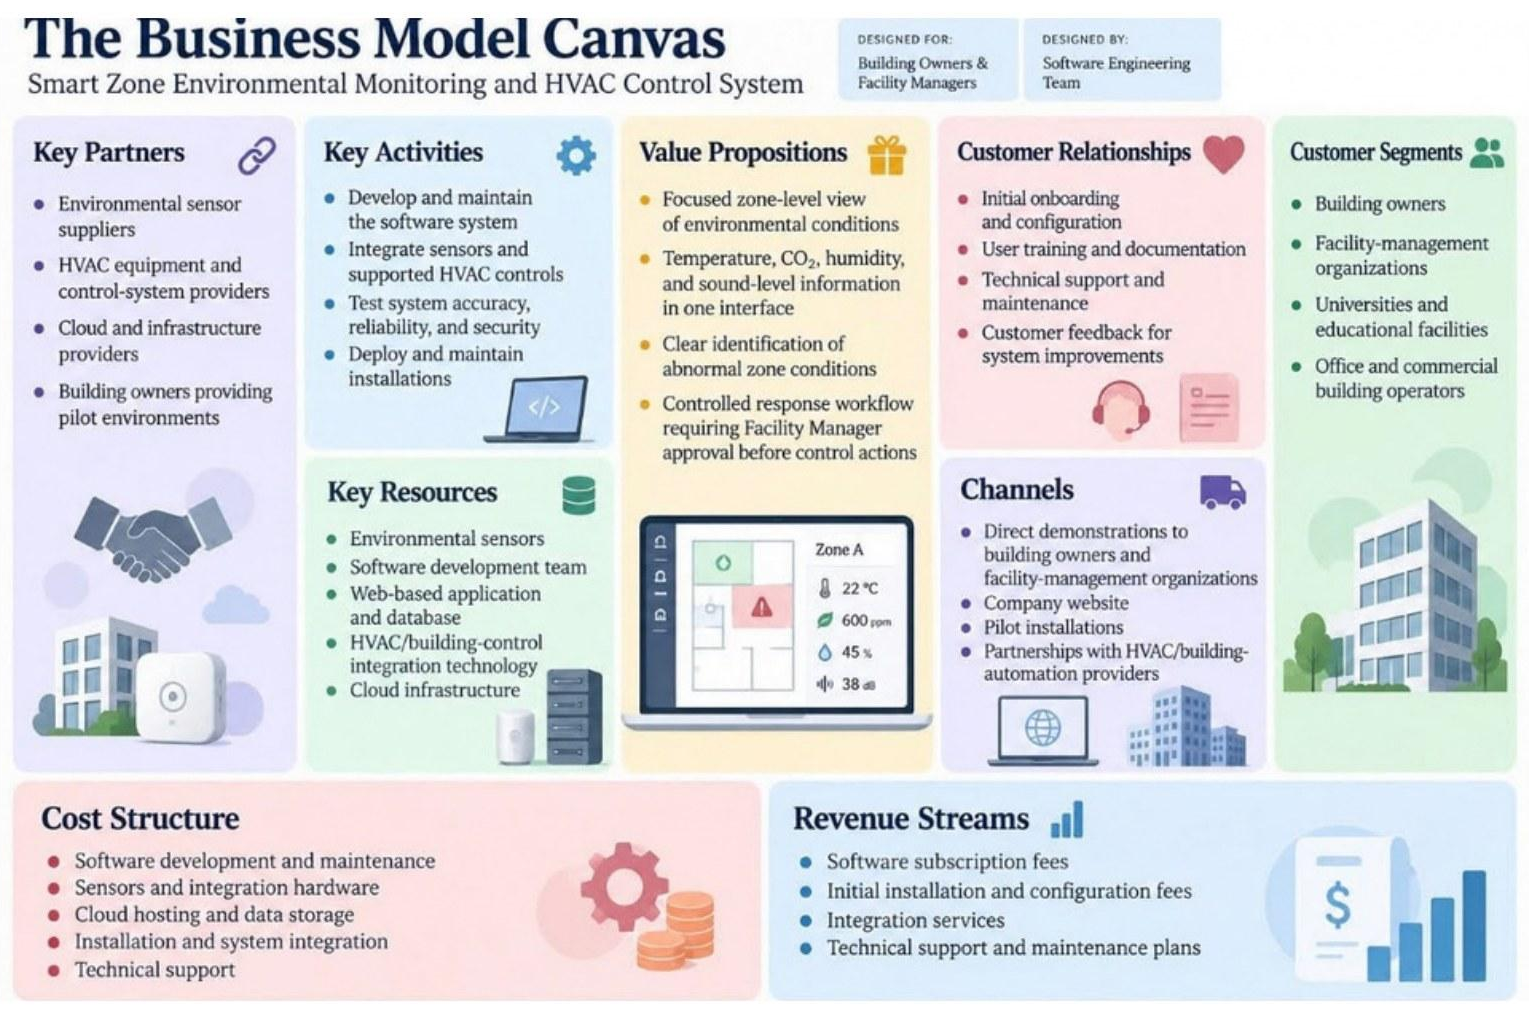
\includegraphics[width=\linewidth]{business_model_canvas.png}
  \caption{Business Model Canvas for ZoneSense}
  \label{fig:bmc}
\end{figure}

% ---------------------------------------------------------------------
\clearpage
\section{Literature Review and Gap Analysis}

\subsection{Purpose and Method}
This section extends the market study (Section~2) with published research. Section~2 described what commercial platforms offer; this section asks \textit{how} existing systems, commercial and academic, work, which problems their authors or users report, and how ZoneSense is designed to respond. Each system is described by what it built and the problem it reports, and the response of ZoneSense is stated next to the problems. The review draws on 12 research studies (listed in the References) and on vendor documentation and public user reviews. Only problems that ZoneSense responds to are listed, and commercial platforms are described from vendor documentation and user reviews, so no failure is claimed for them beyond what those sources state.

\subsection{Environmental Monitoring Systems}
Earlier studies show that environmental sensor systems can be built and run successfully. The problems below are the ones that matter for ZoneSense: readings that go missing, and sound sensing that raises a privacy question.

{\small\stripe
\begin{xltabular}{\linewidth}{|L{3.2cm}|L{5.4cm}|Y|}
\caption{Environmental monitoring studies}\label{tab:env}\\
\hline\headrow
\hd{Study} & \hd{What they built} & \hd{Problem reported}\\\hline
\endfirsthead
\hline\headrow
\hd{Study} & \hd{What they built} & \hd{Problem reported}\\\hline
\endhead
Andriamandimbihasina et al.\ (2025) & 27 sensors from several manufacturers placed in four university classrooms. & A high rate of readings was \textbf{missing}.\\\hline
Du et al.\ (2025) & A simulation of what happens when wireless (LoRaWAN) messages are lost in a cloud-connected building system. & A system that sends a reading \textbf{only when the temperature changes} became very unreliable when messages were lost.\\\hline
Huang, Ge, \& Lu (2016) & A system that estimates how many people are in a room by \textbf{recording the room's sound} with microphones, including recognising individual voices. & The authors say the approach protects privacy, but the paper \textbf{does not describe how the recordings or the learned voice models are stored or protected}.\\\hline
\end{xltabular}}

\keephead{How ZoneSense responds}
\begin{itemize}
\item \textbf{Missing or lost readings} (Andriamandimbihasina et al., 2025; Du et al., 2025). Every sensor reports at least once every 60 seconds (FR2). A sensor that misses 3 reports in a row is marked \textit{unavailable} within 8 seconds (NFR3), and unavailable is shown as its own status, never as a normal value (FR6, NFR9). All other zones keep running (NFR8).
\item \textbf{Sound and privacy} (Huang et al., 2016). ZoneSense stores sound \textit{levels} only and records no audio (NFR10). Huang and Kieffer (2019) took a similar approach: their sensor board kept only the loudness of the sound, so speech could not be recovered.
\end{itemize}

\subsection{Commercial Building Management Platforms}
The four platforms studied in the market analysis already combine environmental measurement, visualisation, alarms and HVAC control, so they show what is technically possible. Siemens Desigo and Building X (Siemens, n.d.-a, n.d.-b) offer automation, energy management and analytics for large portfolios. Johnson Controls Metasys (Johnson Controls, n.d.-a, n.d.-b) centralises monitoring and alarm management across building systems. Schneider Electric EcoStruxure Building Operation (Schneider Electric, n.d.-a) provides dashboards, alarms and system integration. Honeywell's building management solutions (Honeywell, n.d.) add remote and multi-site management. The problems below come from vendor documentation and public user reviews (G2, n.d.-a, n.d.-b, n.d.-c); no failure is claimed beyond what those sources say.

{\small\stripe
\begin{xltabular}{\linewidth}{|L{3.2cm}|L{5.4cm}|Y|}
\caption{Commercial platforms}\label{tab:commercial}\\
\hline\headrow
\hd{Platform} & \hd{What it offers} & \hd{Problem reported}\\\hline
\endfirsthead
\hline\headrow
\hd{Platform} & \hd{What it offers} & \hd{Problem reported}\\\hline
\endhead
Siemens Desigo CC & Automation, HVAC control, alarms and analytics for large building portfolios. & Supervisor approval of commands (the ``Four Eyes'' option) is available for critical objects that have been set up for validation, so it does not cover every control action by default (Siemens, n.d.-c).\\\hline
Johnson Controls Metasys & Centralised monitoring and alarm management. & Some reviewers report limits with graphics, interface usability, response time and the \textbf{initial learning process} (G2, n.d.-c).\\\hline
Schneider Electric EcoStruxure & Dashboards, alarms and integration with HVAC and other systems. & A verified reviewer reported that \textbf{training was required} before becoming comfortable with the system (G2, n.d.-a).\\\hline
Honeywell building management & Monitoring, HVAC control, remote and multi-site management. & Some customer feedback identifies \textbf{cost} as a concern (G2, n.d.-b).\\\hline
\end{xltabular}}

\keephead{How ZoneSense responds}
\begin{itemize}
\item \textbf{Learning effort} (Metasys, EcoStruxure reviewers). ZoneSense is a small system for one building with up to 20 zones (FR1, NFR12). It uses four statuses, shown the same way on every screen (NFR9), so there is less to learn.
\item \textbf{Approval only for configured objects} (Siemens, n.d.-c). In ZoneSense every proposed control action needs the approval of an authorized Building Resident before it runs, with no per-object setup, and 0 actions are executed before approval is recorded (FR10).
\end{itemize}

\subsection{Security and Access Control}
Studies of smart-building security describe layered protection for building systems. These are the problems they report.

{\small\stripe
\begin{xltabular}{\linewidth}{|L{3.2cm}|L{5.4cm}|Y|}
\caption{Security studies}\label{tab:security}\\
\hline\headrow
\hd{Study} & \hd{What they built} & \hd{Problem reported}\\\hline
\endfirsthead
\hline\headrow
\hd{Study} & \hd{What they built} & \hd{Problem reported}\\\hline
\endhead
Ciholas et al.\ (2019) & A systematic review of smart-building security research. & In some real buildings, \textbf{security was never a requirement} when the building was set up, and there was \textbf{no central user management}.\\\hline
Franco et al.\ (2024) & A sensor network that runs on the building's own internal network. & The authors claimed an internal network is safer from attack, but this was \textbf{never tested}.\\\hline
Elsayed et al.\ (2025) & A review of smart building management systems built on connected sensors and automated controls. & Joining sensors, automated controls and networked management in one system brings \textbf{complicated cybersecurity issues}.\\\hline
\end{xltabular}}

\keephead{How ZoneSense responds}
\begin{itemize}
\item \textbf{Security as a requirement, managed in one place} (Ciholas et al., 2019). Every protected function requires a login (FR20, NFR4), every request is checked against the user's role (FR21, NFR5), and approvals, executed actions and maintenance are recorded with the responsible user (NFR6, FR14).
\item \textbf{Trusting the network} (Franco et al., 2024; Elsayed et al., 2025). ZoneSense does not rely on the network being safe. All browser, sensor-gateway and database connections use TLS 1.2 or higher, and passwords are stored hashed (NFR13). No control command is sent without a recorded approval (FR10).
\item \textbf{Design reference.} Rathinavel et al.\ (2017) describe a secure building platform with hashed passwords, TLS, sessions and three roles. ZoneSense follows the same layered idea, with all access passing through one access layer.
\end{itemize}

\subsection{Automation and Human Oversight}
Recent research applies machine learning to building control. In these studies ``human in the loop'' usually means that the AI learns from occupant comfort feedback or explains its output to managers, not that a person approves each action.

{\small\stripe
\begin{xltabular}{\linewidth}{|L{3.2cm}|L{5.4cm}|Y|}
\caption{AI-assisted control and oversight}\label{tab:ai}\\
\hline\headrow
\hd{Study} & \hd{What they built} & \hd{Problem reported}\\\hline
\endfirsthead
\hline\headrow
\hd{Study} & \hd{What they built} & \hd{Problem reported}\\\hline
\endhead
Muthu Bharath et al.\ (2026) & An explainable digital twin (a digital model of the building kept up to date with real data) with dashboards for different roles. & The AI plan \textbf{failed in 24\% of trials without a clear explanation}.\\\hline
Pritoni et al.\ (2022) & Automatic fault-correction routines added to two commercial tools and tried in four buildings. Users could approve each correction or switch to automatic correction. & Users raised concerns about \textbf{accountability and loss of control}.\\\hline
Fatehi Karjou et al.\ (2025) & Reinforcement learning (an AI method that learns from feedback about earlier decisions) for smart radiator valves in a real office. & \textbf{Communication delays} caused problems.\\\hline
\end{xltabular}}

\keephead{How ZoneSense responds}
\begin{itemize}
\item \textbf{Unexplained decisions} (Muthu Bharath et al., 2026). ZoneSense uses clear threshold rules that an authorized Building Resident can read and change without editing code (FR5, NFR11).
\item \textbf{Accountability and control} (Pritoni et al., 2022). Every control action needs approval before it runs (FR10), and every approval or rejection is recorded with the responsible user and the time (FR14, NFR6).
\item \textbf{Delays} (Fatehi Karjou et al., 2025). ZoneSense sets time limits: an alert within 45 seconds (FR7, NFR2), a proposed action within 10 seconds (FR9) and an approved action sent within 2 seconds (FR12).
\end{itemize}

\subsection{Alert Overload}
A monitoring system also has to avoid alerting too often, because people stop responding to alerts that keep repeating.

{\small\stripe
\begin{xltabular}{\linewidth}{|L{3.2cm}|L{5.4cm}|Y|}
\caption{Alert overload}\label{tab:alerts}\\
\hline\headrow
\hd{Study} & \hd{What they built} & \hd{Problem reported}\\\hline
\endfirsthead
\hline\headrow
\hd{Study} & \hd{What they built} & \hd{Problem reported}\\\hline
\endhead
Li et al.\ (n.d.) & A study of the building automation system of a university building complex at Carnegie Mellon University, including interviews with facility managers. & One of the campus's six systems produced \textbf{over 610,000 alarms}. The most frequent were ``zone temperature abnormal'' and ``normal'' alarms, which \textbf{repeated whenever a zone's temperature moved around a threshold} and did not mean an equipment fault. Facility managers acknowledged them without inspection, or ignored them, which risked missing severe alarms.\\\hline
\end{xltabular}}

\keephead{How ZoneSense responds}
\begin{itemize}
\item \textbf{Repeated alarms} (Li et al., n.d.). The first alert is always shown within 45 seconds (FR7, NFR2). The authorized Building Resident sets a repeat-alert interval of 1 to 60 minutes (default 10) for each zone and measurement (FR22). Repeats of an unchanged condition inside the interval are not shown again, but 100\% of them are stored in the alert history, and a worse severity always raises a new alert (FR22).
\end{itemize}

\subsection{Gap Analysis and ZoneSense Response}
Each gap below is a problem reported in the sources above, followed by what ZoneSense does about it and the requirements that carry the response.

{\small\stripe
\begin{xltabular}{\linewidth}{|C{0.7cm}|L{4.6cm}|Y|L{2.7cm}|}
\caption{Gap, response and requirement}\label{tab:gap}\\
\hline\headrow
\hd{No.} & \hd{Gap in previous systems} & \hd{ZoneSense response} & \hd{Requirements}\\\hline
\endfirsthead
\hline\headrow
\hd{No.} & \hd{Gap in previous systems} & \hd{ZoneSense response} & \hd{Requirements}\\\hline
\endhead
1 & Readings that go missing, are lost or arrive late (Andriamandimbihasina et al., 2025; Du et al., 2025; Fatehi Karjou et al., 2025). & A sensor that misses 3 consecutive 60-second intervals is marked unavailable within 8 seconds, a failing sensor never interrupts other zones, and alerts and commands have time limits. & FR2, FR7, FR9, FR12, NFR3, NFR8, NFR9\\\hline
2 & Automated control that is hard to explain and leaves accountability unclear (Muthu Bharath et al., 2026; Pritoni et al., 2022). & Transparent threshold rules; every proposed action needs approval by an authorized Building Resident before it runs; each decision is recorded with the responsible user. & FR5, FR10, FR14, NFR6, NFR11\\\hline
3 & Security not treated as a requirement, and an untested belief that an internal network is safe (Ciholas et al., 2019; Franco et al., 2024; Elsayed et al., 2025). & Login and a role check on every protected function with audit records, and ZoneSense adds TLS 1.2 or higher on all connections with hashed passwords. & FR14, FR20, FR21, NFR4--NFR6, NFR13\\\hline
4 & Sound sensing that records audio without explaining how it is protected (Huang et al., 2016). & Only sound-level values are processed and stored; 0 audio recordings. & NFR10\\\hline
5 & Commercial platforms: reviewers report learning effort and cost, and supervisor approval is an option for configured objects (G2, n.d.-a, n.d.-b, n.d.-c; Siemens, n.d.-c). & A focused system for up to 20 zones in one building, four statuses used on every screen, and mandatory approval for every control action. & FR1, FR10, NFR9, NFR12\\\hline
6 & Too many repeated alerts that people acknowledge or ignore (Li et al., n.d.). & ZoneSense adds a configurable repeat-alert interval: the first alert is always shown within 45 seconds, repeats of an unchanged condition are stored but not re-notified, and a worsening severity always raises a new alert. & FR22, FR7, NFR2\\\hline
\end{xltabular}}

\textbf{Limits of this review.} The review draws on 12 research studies and on vendor documentation and public user reviews, so its conclusions apply to those sources and not to the whole field. Some studies are small, such as a single laboratory or one building, or were run in simulation, so their problems may look different elsewhere. Only problems that ZoneSense responds to are listed, so this is not a complete account of every weakness in these studies. ZoneSense is a prototype with simulated sensors and HVAC equipment; this review shows how its requirements respond to reported gaps, and it does not claim that ZoneSense has been validated against the systems reviewed.

\begin{zcallout}
\textbf{Resulting requirements (Lab 3, Sections 1.1 and 1.2): FR22} (repeat-alert interval, from gap 6) and \textbf{NFR13} (encrypted transport, from gap 3).
\end{zcallout}

% ---------------------------------------------------------------------
\clearpage
\section*{References}
\addcontentsline{toc}{section}{References}
\begingroup\small
\setlength{\parindent}{-1.5em}\setlength{\leftskip}{1.5em}\setlength{\parskip}{5pt}\raggedright

Andriamandimbihasina, I., Gallego, S., \& Lartigue, B. (2025). Insightful settings of indoor environmental sensors implementation for effective building data analysis: A case study of university classrooms. \textit{Journal of Physics: Conference Series, 3140}, 052008. \url{https://doi.org/10.1088/1742-6596/3140/5/052008}

Ciholas, P., Lennie, A., Sadigova, P., \& Such, J. M. (2019). The security of smart buildings: A systematic literature review. arXiv:1901.05837 [preprint].

Du, J., Jiang, J., Yuan, B., Streblow, R., \& M\"uller, D. (2025). Impact of LoRaWAN wireless communication on reliability of cloud-based building automation systems. \textit{Journal of Physics: Conference Series, 3140}, 042005. \url{https://doi.org/10.1088/1742-6596/3140/4/042005}

Elkafrawy, P. (2026). \textit{CS3151 Software Engineering -- Fall 2026 course syllabus}. Effat University.

Elsayed, R., Ismail, M. I., Ashour, A. F., Sakr, H. A., Ibrahem, M. I., \& Fouda, M. M. (2025). A review of smart building management systems: CPS applications for energy-efficient monitoring and control. IEEE AIBThings 2025. \url{https://doi.org/10.1109/AIBThings66987.2025.11296174}

Fatehi Karjou, P., Stupperich, F., Stoffel, P., \& M\"uller, D. (2025). Human-in-the-loop control strategy for IoT-based smart thermostats with deep reinforcement learning. \textit{Energy and AI, 20}, 100490. \url{https://doi.org/10.1016/j.egyai.2025.100490}

Franco, A., Crisostomi, E., Dalmiani, S., \& Poletti, R. (2024). Synergy in action: Integrating environmental monitoring, energy efficiency, and IoT for safer shared buildings. \textit{Buildings, 14}(4), 1077. \url{https://doi.org/10.3390/buildings14041077}

G2. (n.d.-a). \textit{EcoStruxure reviews}. \url{https://www.g2.com/products/ecostruxure/reviews}

G2. (n.d.-b). \textit{Honeywell Intelligent Buildings reviews}. \url{https://www.g2.com/products/honeywell-intelligent-buildings/reviews}

G2. (n.d.-c). \textit{Metasys reviews}. \url{https://www.g2.com/products/metasys/reviews}

Honeywell. (n.d.). \textit{Building management solutions}. \url{https://buildings.honeywell.com/us/en/solutions/buildings.html}

Huang, Q., Ge, Z., \& Lu, C. (2016). \textit{Occupancy estimation in smart buildings using audio-processing techniques} [Preprint]. arXiv. \url{https://arxiv.org/abs/1602.08507}

Huang, Q., \& Kieffer, K. (2019). An intelligent Internet of Things (IoT) sensor system for building environmental monitoring. \textit{Journal of Mobile Multimedia, 15}(1-2), 29-50. \url{https://doi.org/10.13052/jmm1550-4646.15122}

Johnson Controls. (n.d.-a). \textit{Metasys building automation system}. \url{https://www.johnsoncontrols.com/building-automation-and-controls/building-management/building-automation-systems-bas/metasys-software-and-servers}

Johnson Controls. (n.d.-b). \textit{Metasys user interface and alarm management documentation}. \url{https://docs.johnsoncontrols.com/bas/r/Metasys}

Li, H., Aziz, A., Cochran, E., \& Lasternas, B. (n.d.). \textit{Building automation system alarm management for operation and maintenance decision making} [Conference paper]. Center for Building Performance and Diagnostics, Carnegie Mellon University.

Muthu Bharath, J., Balamurugan, S., Thomas, N. S., \& Gnana Swathika, O. V. (2026). AI-driven explainable digital twin with adaptive decision support for multi-zone smart buildings. \textit{Discover Sustainability, 7}, 1046. \url{https://doi.org/10.1007/s43621-026-03394-4}

Pritoni, M., Lin, G., Chen, Y., Vitti, R., Weyandt, C., \& Granderson, J. (2022). From fault-detection to automated fault correction: A field study. \textit{Building and Environment, 214}, 108900. \url{https://doi.org/10.1016/j.buildenv.2022.108900}

Rathinavel, K., Pipattanasomporn, M., Kuzlu, M., \& Rahman, S. (2017). Security concerns and countermeasures in IoT-integrated smart buildings. In \textit{2017 IEEE Power \& Energy Society Innovative Smart Grid Technologies Conference} (ISGT). IEEE. \url{https://doi.org/10.1109/ISGT.2017.8086057}

Schneider Electric. (n.d.-a). \textit{EcoStruxure Building Operation}. \url{https://www.se.com/uk/en/product-range/62111-ecostruxure-building-operation/}

Schneider Electric. (n.d.-b). \textit{Workplace and building environmental management solutions}. \url{https://www.se.com/sa/en/product-range/117451134-planon-workplace/\#overview}

Siemens. (n.d.-a). \textit{Building X and building automation solutions}. \url{https://www.siemens.com/en-us/products/building-x/}

Siemens. (n.d.-b). \textit{Desigo room units and sensors}. Siemens Building Products. \url{https://www.siemens.com/us/en/products/buildingtechnologies/automation/desigo-room-operation-units.html}

Siemens. (n.d.-c). \textit{Configuring validation}. In \textit{Desigo CC engineering help}. \url{https://gbscampus.vu.nl/WebApp/Help/EngineeringHelp/en-US/17985449611.html}

\endgroup
\end{document}
